\section{Problem Formulation}
\label{sec:problem}
In this section, we first introduce mathematical notations. Then we formalize our approach to group anomaly.
We first describe the accompanying notations in section~\ref{sec:notations} which will be used throughout the chapter.
Then we formally present problem statement, provide a brief comparison of our approach to conventional solutions, and review the challenging issues that are relevant to event detection problem.
\subsection{Notations}
\label{sec:notations}
Given an undirected, weighted graph $\mathbf{G}(V,E;f)$, where $V=\{v_0,v_1,...,v_{N-1}\}$ represents the set of $N$ cities, $E$ refers to the connections between neighboring cities. $W$ is a matrix of non-negative weights associated with each edge, where $e_{ij}\in E$. The function, $f: V \rightarrow {\mathbb{R}}^N$ maps the vertices of graph $\mathbf{G}$, and $f(n)$ stands for the value on the vertex $v_n$. Graph $\mathbf{G}$'s adjacency matrix $\mathbf{A}$ is of size $N\times N$, where each element $a_{ij}$ is represented as:
\begin{equation}
a_{ij} = \left\{ \begin{array}{rl}
 w_{ij} &\mbox{ when $e_{ij}\in {E}$} \\
  0 &\mbox{ otherwise}
       \end{array} \right.
\end{equation}
Here, $\mathbf{A}$ is symmetric since $a_{ij}=a_{ji}$.
Let $d_i=\sum\limits_{v_j \in V}a_{ij}$ be the sum of all edge weights that are incident on $v_i$, and $\mathbf{D}$ be the diagonal matrix denoted as $\mathbf{D}=diag\{d_1,d_2,\ldots,d_N\}$. A Laplacian matrix $\mathcal{L}$ is defined as $\mathcal{L}=\mathbf{D-A}$. It is a symmetric matrix and has real eigenvalues $\lambda_{i}$ such that $0 = \lambda_{0} < \lambda_{1} \leq \lambda_{2} \leq \ldots \leq \lambda_{N-1} = \lambda_{max}$. The complete set of $\mathcal{L}$'s normalized eigenvectors~\cite{bapat2010graphs} $\chi_{i}$ for $i=0,1,2,...,N-1$ is described as:
\begin{equation}
\label{eq:eigenvalues}
\mathcal{L}\chi_{i}=\lambda_{i}\chi_{i}
\end{equation}
The set of eigenvalue and normalized eigenvector pair is denoted as:
\begin{equation}
\label{eq:eigenvalues}
\sigma({\mathbf{G}}):=\{(\lambda_l,\chi_l)\}_{l=0}^{N-1}.
\end{equation}$\sigma({\mathbf{G}})$ is also called graph spectral of $\mathbf{G}$.




\subsection{Problem Statement}
\label{sec:problemformulation}
In this chapter, we focus on the problem of group anomaly from online social networks, based on the absenteeism behavior observed in user activity in geographically proximal communities or group of cities.
Conventionally, this problem can be described as following: \emph{given a graph and \textit{absenteeism score} vector, $\mathbf{G}(V,E;f^t)$ at time interval $t$, select a subset $\Sigma \subseteq V$, such that
\begin{eqnarray}
 \label{eq: problem}
    \Sigma=\underset{P\subseteq V, P \mbox{ is compact}}{\arg\min}\ \ \sum_{v_k\in P} {f(k)}
\end{eqnarray} }
However, how to define compactness of the selected subset $\Sigma$ is an open problems.
A general solution to this problem is employing a combinatorial optimization method, by defining a constrained objective function over a network one can identify a subset of vertices which maximize the corresponding function~\cite{rozenshtein2014event}. Therefore, Equation~\ref{eq: problem} can be modified as:
\begin{eqnarray}
 \label{eq: problem_conventional}
    \Sigma=\underset{P\subseteq V}{\arg\min}\ \ \sum_{v_k\in P} {f(k)}+\lambda \mu(P)
\end{eqnarray}
, where $\mu(P)$ is the compactness penalty function of $P$ (e.g., the sum of distances among
all pairs of the vertices in $P$~\cite{rozenshtein2014event}), and $\lambda$ is the regularization parameter.
Such methods suffer from the following issues:
\begin{enumerate}
\item To define and measure the compactness of subset $P\subseteq V$ is challenging, considering the exponential varieties of complex graphs.
\item To determine a suitable regularization parameter $\lambda$ in the objective function is ambiguous, because simply combining multiple physical different concepts in the objective function makes the optima sensitive to $\lambda$.
\item To solve this objective function is often a NP-hard problem, which makes it unpractical in many real world applications. Sometimes, even the approximate solutions are of high computation complexity, if there are any.
\end{enumerate}
In contrast, our approach proposes a novel group anomaly algorithm in social networks using spectral graph wavelet theory.
The graph wavelets focus on the intrinsic geometric structure of the graph by transforming each vertex $v_i\in V$, and mining the topological information of both local and global centered vertices to support multiscale analysis.
In addition, the graph wavelet approach identifies anomaly group which is automatically compact, and provides a fair and low computational method in terms of complexity for identifying abnormal group behavior in a broad application scenarios.



\begin{figure}[h]
	\centering
    {
		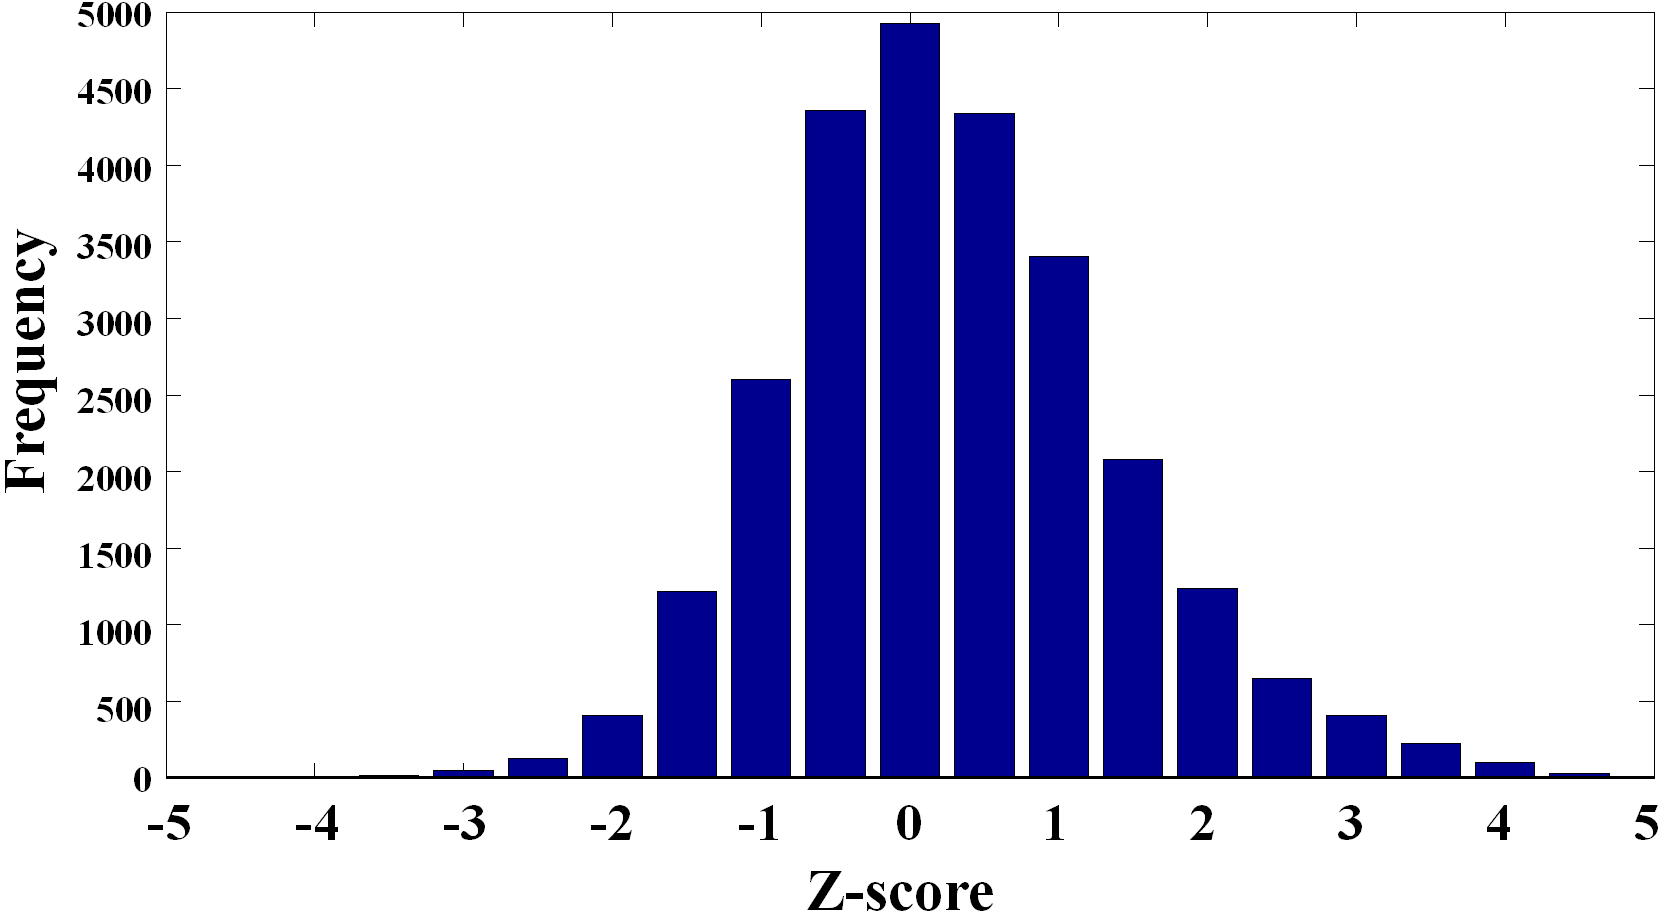
\includegraphics[width=3in] {figures/Z-Score-distribution.png}
		\label{fig:distribution}
	}
	\caption{ Z-score distribution of city Sao Paulo, Brazil from Aug 1, 2012 to January 30, 2014 with time interval of five minutes. }
	\label{fig:zscore-distribution}
\end{figure}
